\documentclass{article}
\usepackage[utf8]{inputenc}
\usepackage[english]{babel}
\usepackage{graphicx}
\usepackage{amsmath}
\usepackage[backend=biber,sorting=none]{biblatex}
\usepackage{geometry}
\addbibresource{mybib.tex}

\title{Dynamical Neural Network Models\\for Sequence Learning}
\author{Sharath Ramkumar\\
Advisor: Dr. Robert Kozma\\University of Massachusetts Amherst\\COMPSCI 496: Independent Study}
\date{}

\begin{document}
\maketitle

\begin{abstract}
In this study, we explore various neural network models for learning sequences. We also propose alternative dynamic spiking neural architectures and compare accuracy and robustness of these network models to randomized temporal noise on a artificial prediction task.
\end{abstract}

\section*{Introduction}

Neural network models are able to achieve superhuman performance on static tasks through recent breakthroughs in deep learning. However, the majority of real-world time-series data is often complex and noisy. As a result, we need dynamic models that can adapt to changing data streams to learn and predict in an robust, semi-supervised fashion. 

\section*{Background}
There have been some recent studies comparing various models for time-series prediction tasks \cite{cui2016continuous} on discretized data. In this study, we will replicate their results to establish a baseline and propose unsupervised spiking neural architectures for performing this task. Spiking neurons \cite{gerstner2002spiking} are biologically-inspired models of neurons. Spiking neural networks (SNNs) \cite{maass1997networks} are organized connections between these spiking neurons which have more energy efficient \cite{cruz2012energy} implementations on neuromorphic hardware.

\section*{Methodology}

\subsection*{Artificial Dataset}

Cui et al. (2016) propose an artificial dataset of sequences (formed with characters) with overlapping subsequences. A sequence is sampled from the dataset and presented to the model at each time step. After the last character of the sequence is presented, a character is sampled from the noise distribution and shown to the model. This process is repeated until $10,000$ characters (counting both sequences and noise characters) are shown to the model. After the model sees $10,000$ characters, the last character of sequences with shared subsequences is swapped. The performance on this task is the accuracy of predicting the last character over a window of the last $100$ sequences. A sample dataset is summarized in Table \ref{tab:dataset}.

\begin{table}[!h]
    \centering
    \begin{tabular}{|c|c|} \hline
        Pre-$10,000$ & Post-$10,000$  \\ \hline
        \begin{tabular}{|c|c|c|}
            Start & Subsequence & End \\ \hline
            $6$ & $8, 7, 4, 2, 3$ & $0$ \\ \hline
            $1$ & $8, 7, 4, 2, 3$ & $5$ \\ \hline
            $6$ & $3, 4, 2, 7, 8$ & $5$ \\ \hline
            $1$ & $3, 4, 2, 7, 8$ & $0$ \\ \hline
            $0$ & $9, 7, 8, 5, 3, 4$ & $1$ \\ \hline
            $2$ & $9, 7, 8, 5, 3, 4$ & $6$ \\ \hline
            $0$ & $4, 3, 5, 8, 7, 9$ & $6$ \\ \hline
            $2$ & $4, 3, 5, 8, 7, 9$ & $1$ \\ \hline
        \end{tabular} &  \begin{tabular}{|c|c|c|}
            Start & Subsequence & End \\ \hline
            $6$ & $8, 7, 4, 2, 3$ & $5$ \\ \hline
            $1$ & $8, 7, 4, 2, 3$ & $0$ \\ \hline
            $6$ & $3, 4, 2, 7, 8$ & $0$ \\ \hline
            $1$ & $3, 4, 2, 7, 8$ & $5$ \\ \hline
            $0$ & $9, 7, 8, 5, 3, 4$ & $6$ \\ \hline
            $2$ & $9, 7, 8, 5, 3, 4$ & $1$ \\ \hline
            $0$ & $4, 3, 5, 8, 7, 9$ & $1$ \\ \hline
            $2$ & $4, 3, 5, 8, 7, 9$ & $6$ \\ \hline
        \end{tabular}\\ \hline
    \end{tabular}
    \caption{A sample artificial dataset for this task. The ending character can be predicted by learning the mapping from the start character and the first character of the shared subsequence to the end character.}
    \label{tab:dataset}
\end{table}

\begin{figure}[!h]
    \centering
    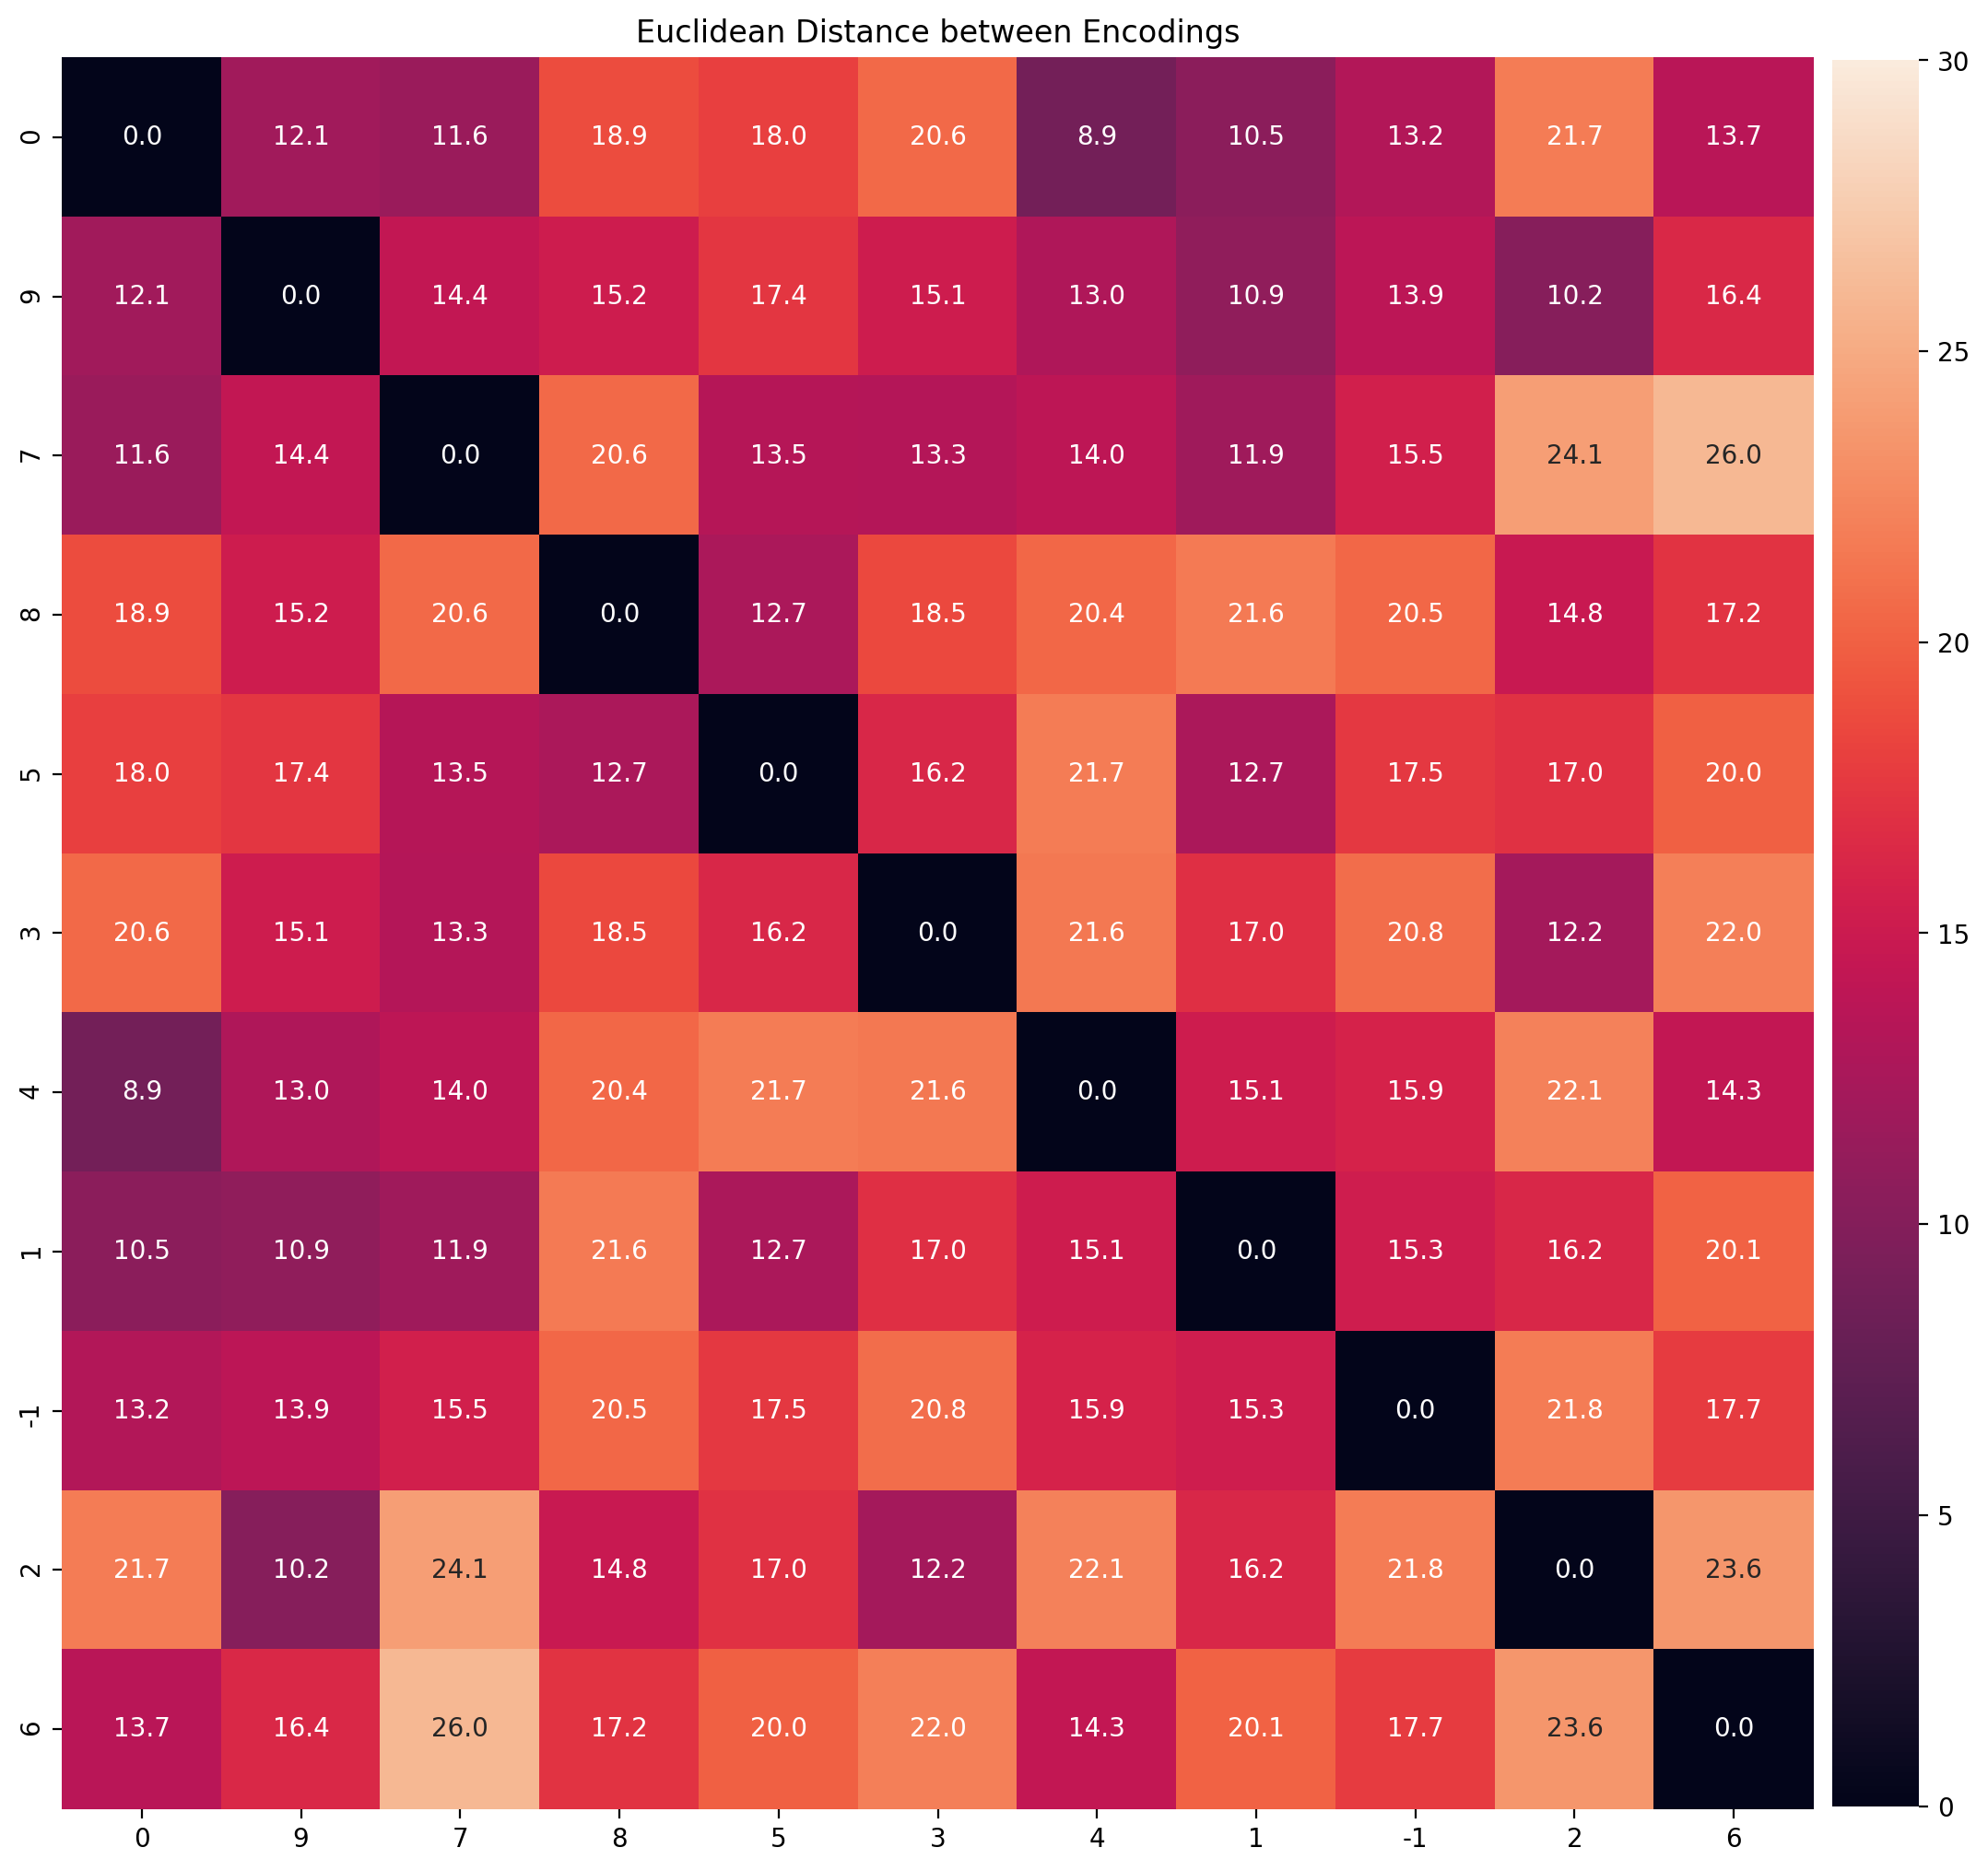
\includegraphics[width=0.7\linewidth]{../notebooks/matrix-distances.png}
    \caption{Heatmap of squared errors between distributed random encodings for the sequence characters, with $-1$ as the separating bit for ease of visualization.}
    \label{fig:encoding-distance}
\end{figure}

\subsection*{Input Encoding}

To present each of these discrete categories to the model, we have to encode the categories to a vector representations. One possibility is to one-hot encode each character, but this representation scales poorly when the number of unique characters increases. For this reason, the characters are encoded as random vectors with real values in the interval $\left[-1, 1\right]$, similar to distributed representations used in natural language learning. \cite{mikolov2013distributed} The euclidean distances between pairs of unique sequence characters using a $25$ length random ending is shown in Figure \ref{fig:encoding-distance}. The decoder for converting vectors back to character uses a nearest neighbor approach, therefore the precision in the output vector from the model is important as the number of noise characters increases. 

\section*{Models}

\subsection*{Long short-term memory networks (LSTM)}

Long short-term memory \cite{hochreiter1997long} networks are able to achieve state of the art results on various sequence learning tasks, so they are a good starting point to establish baseline performance on this task. We use the same LSTM architecture proposed by Cui et al. (2016) with $25$ input neurons connected to a hidden layer of $20$ LSTM cells and $25$ output neurons. The network is trained using truncated backpropagation through time (TBPTT) \cite{mozer1995focused, sutskever2013training} on the last $100$ seen elements. The output is classified using the nearest neighbor decoder.

\subsubsection*{Long short-term memory (LSTM) Behavior}
There are many different variants of LSTM implementations. In this work, the LSTM cell has a forget gate, but no peephole connections. The equations defining the forward pass of the hidden layer in the LSTM model are:

\begin{align*}
    i_t &= \sigma\left(W_{ii}x_t + W_{hi}h_{t-1} + b_i\right)\\
    f_t &= \sigma\left(W_{if}x_t + W_{hf}h_{t-1} + b_f\right)\\
    g_t &= \tanh\left(W_{ig}x_t + W_{hg}h_{t-1} + b_g\right)\\
    o_t &= \sigma\left(W_{io}x_t + W_{ho}h_{t-1} + b_o\right)\\
    c_t &= c_{t-1}\ast f_t + i_t \ast g_t\\
    h_t &= o_t \ast \tanh\left(c_t\right)\\
\end{align*}

In the above equations, $\sigma$ is the sigmoid activation function, $i_t$ is the input gate, $f_t$ is the forget gate, $g_t$ is the cell gate, $o_t$ is the output gate and the $c_t$ and $h_t$ are the cell and hidden states respectively. The $\ast$ operator is the elementwise product operator. The biases $\left(b_i, b_f, b_g, b_o\right)$ and weights $\left(W_{ii}, W_{hi}, W_{if}, W_{hf}, W_{ig}, W_{hg},W_{io}, W_{ho}\right)$ are initialized uniformly from $\left[-\frac{1}{\sqrt{k}}, \frac{1}{\sqrt{k}}\right]$, where $k$ is the number of hidden units. \cite{jozefowicz2015empirical} 

\begin{figure}[!h]
    \centering
    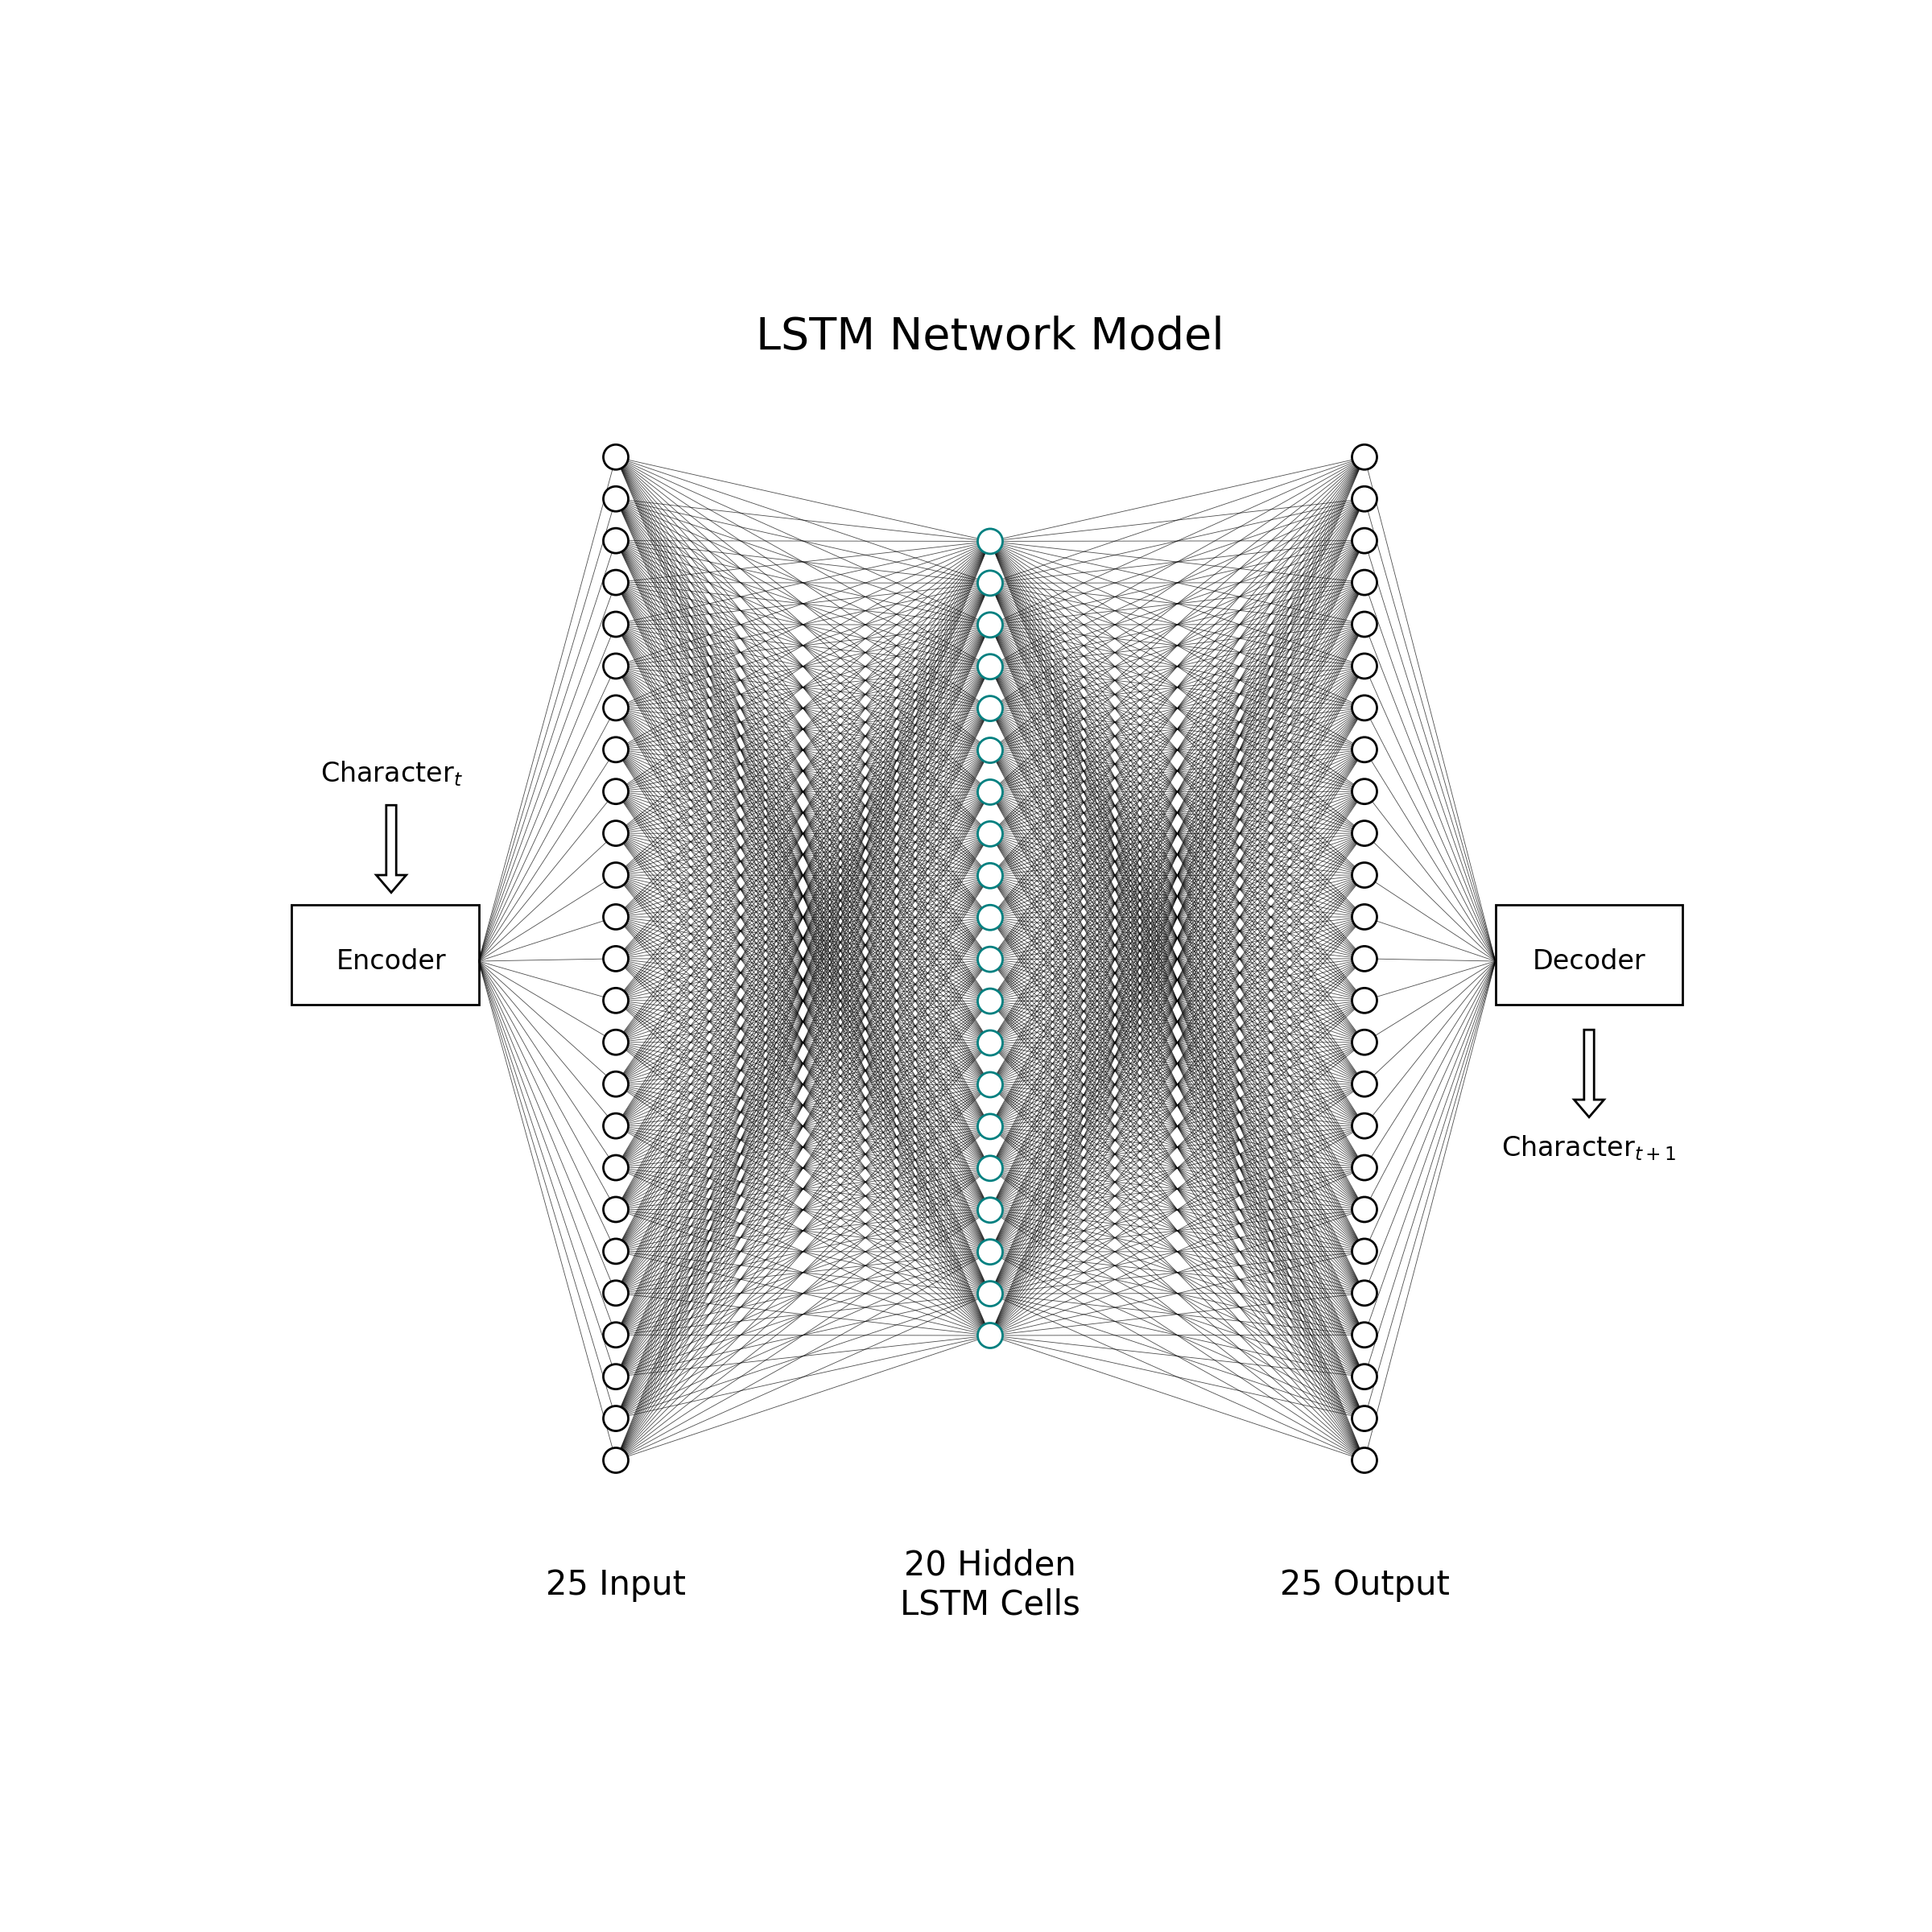
\includegraphics[width=0.9\linewidth]{../diagrams/lstm.png}
    \caption{The network architecture for the LSTM-online model. The LSTM cells maintain an internal hidden state.}
    \label{fig:lstm-online-model}
\end{figure}

\subsection*{Time-delay neural networks (TDNN)}

Time-delay neural networks (TDNN) are feed-forward neural networks trained using a lag on a window of previous data. \cite{waibel1995phoneme} For this task, the TDNN is trained on the last $3000$ samples every $1000$ elements with a lag of $10$. \cite{rojas1996backpropagation} The model has $250$ input neurons that are fully connected to a hidden layer of $200$ neurons. The hidden layers utilize the ReLU non-linearity and are fully connected to $25$ output neurons. The model proposed by Cui et al. has a sigmoid non-linearity in the hidden layer. We replaced the non-linearity to allow for conversion into a spiking neural network. As with the LSTM model, the output is classified using the nearest neighbor decoder.

\begin{figure}[!h]
    \centering
    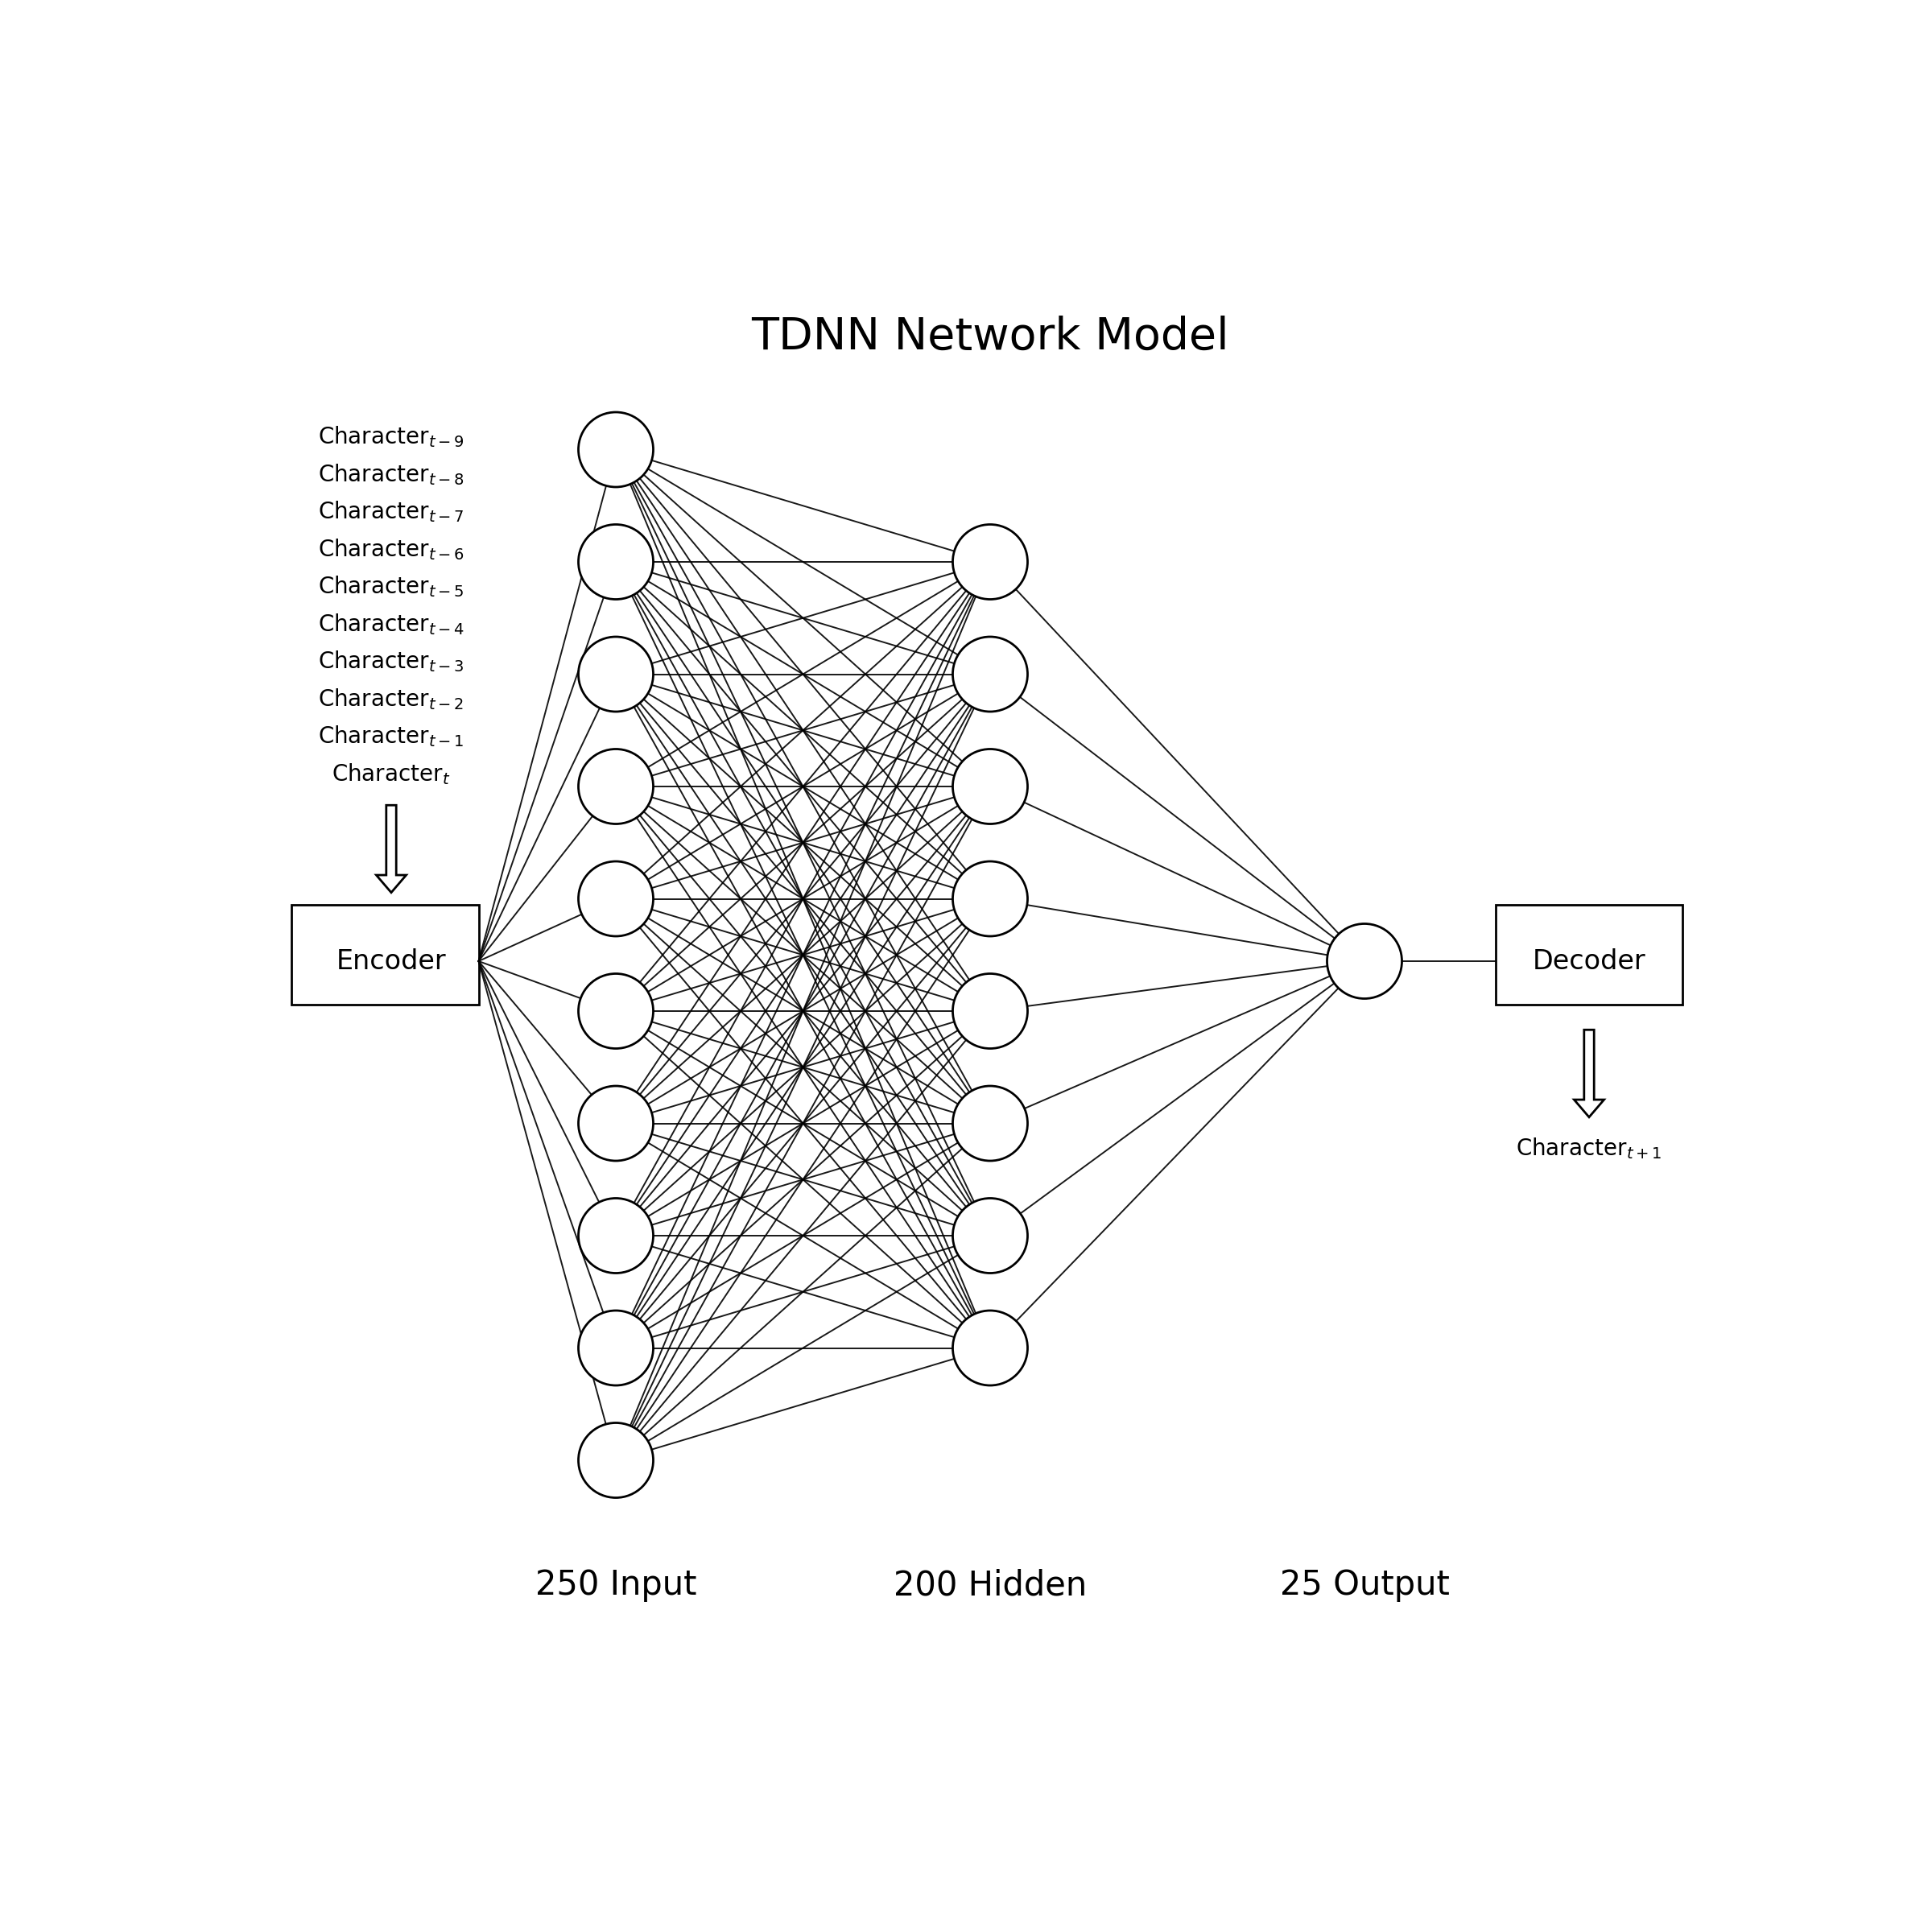
\includegraphics[width=0.9\linewidth]{../diagrams/tdnn.png}
    \caption{The network architecture for the TDNN/TDSNN model.}
    \label{fig:lstm-online-model}
\end{figure}

\subsection*{Time-delay spiking neural networks (TDSNN)}

A common approach to training spiking neural networks is through the transfer of weights learned through backpropagation on an identical non-spiking neural network and then scaling the weights. \cite{diehl2015fast} Using this approach, we can convert the TDNN model trained with backpropagtion into an equivalent spiking network using the approach developed by Diehl et al. (2016)

This method works reasonably well when the output values of the network are positive, however the output has values that are negative. To facilitate these negative spikes, the output layer was doubled in size and the negative weight matrix of the original connections was concatentated. The same was done for the bias. The positive sum of spikes was subtracted from the negative sum of spikes and then divided by the runtime to obtain an approximation of the original network's output.

The drawback of using this method when we need to approximate real-values is the loss of precision based on the duration of the input. For this task, we show the input for $500$ simulated milliseconds. As with the other models, the output is classified using the nearest neighbor decoder.

%\subsection*{K-Nearest Neighbor (KNN)}

\subsection*{Columnar Spiking Neural Network (CSNN)}

While conversion is one way to train a neural network, it is not energy efficient to perform backpropagation and then convert. We propose a spiking neural network architecture, with $10$ inputs, each fully connected to $1$ of $10$ columns of $100$ spiking neurons with randomly initialized weights. Each of the columns has a Hebbian connection to each of the other columns initialized with zero weights. To map the spikes from this network, we train a K-Nearest Neighbor model using previous spikes and values. \cite{beliaev2007time} The model diagram is shown in Figure \ref{fig:csnn-network-diagram}.

\begin{figure}[!h]
    \centering
    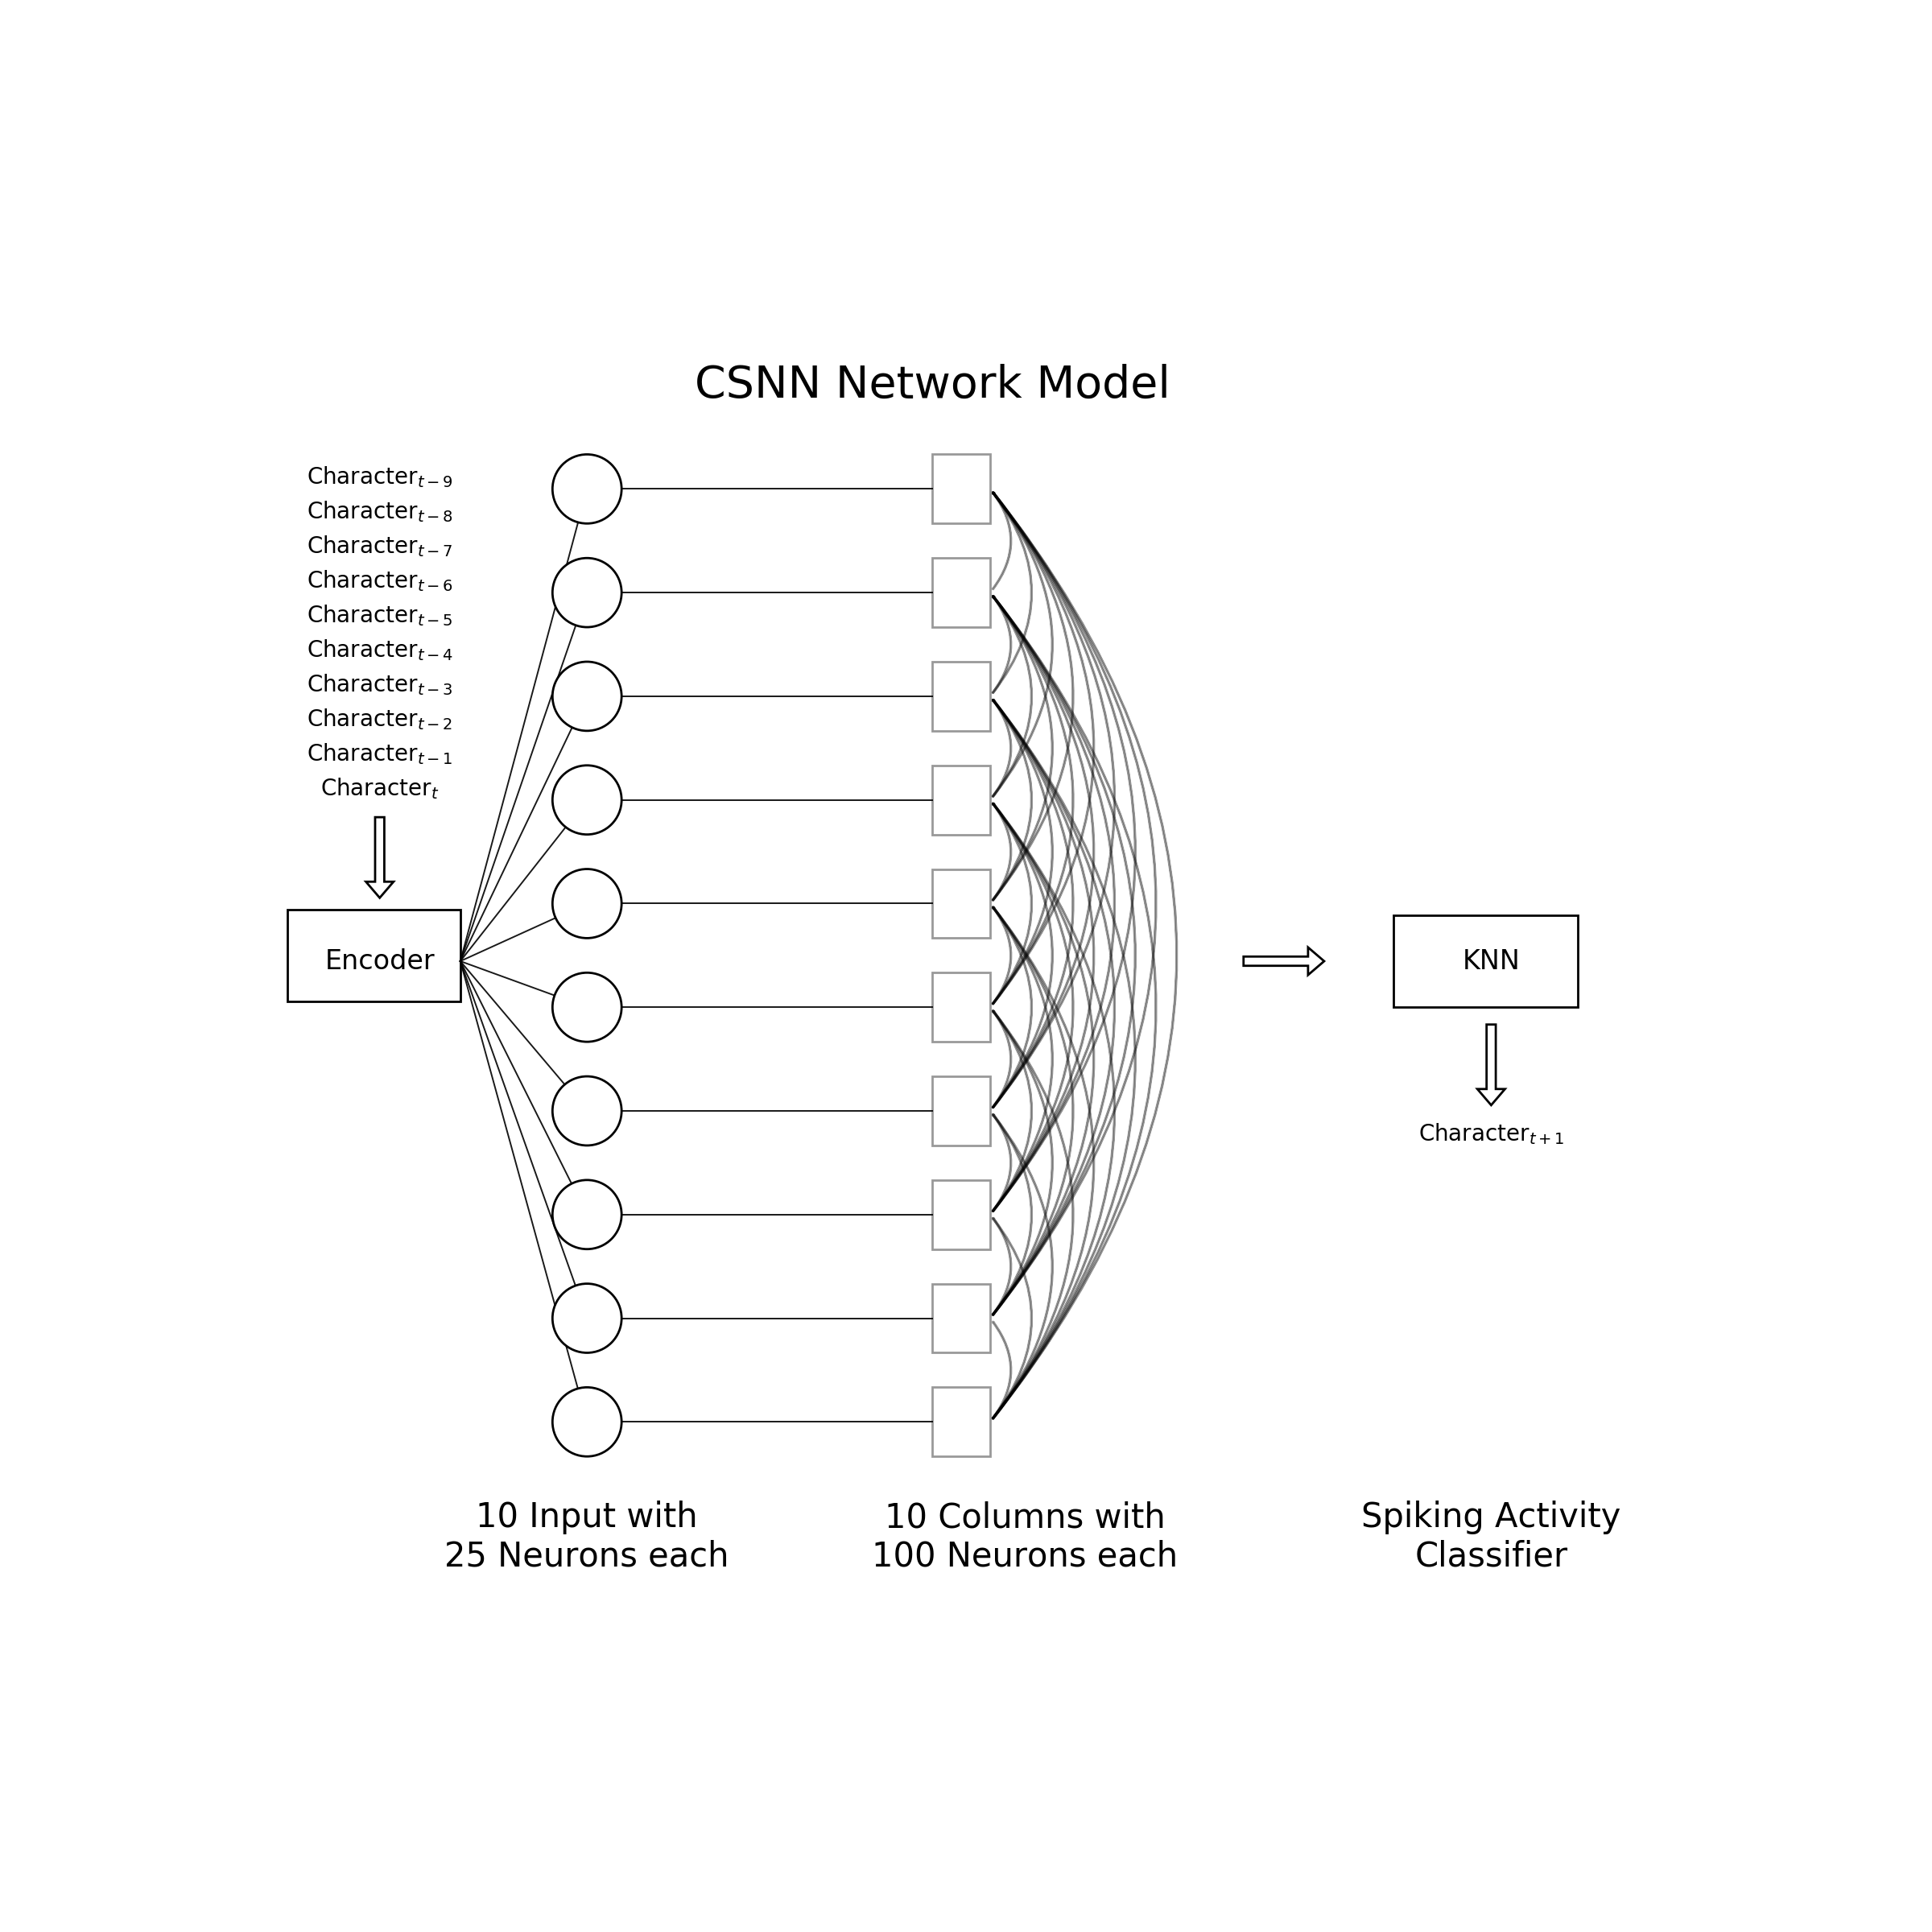
\includegraphics[width=0.9\linewidth]{../diagrams/csnn.png}
    \caption{The network architecture for the CSNN model.}
    \label{fig:csnn-network-diagram}
\end{figure}

\subsubsection*{Hebbian Learning Rule}
The Hebbian learning rule for the CSNN model is defined in terms of the spiking activity of its $k$ columns. The weight change on spike in a connection from column $i$ to column $j$ is defined as follows:

\begin{equation}
    \Delta w_{ij} = \eta(s_{i} - \Tilde{s})(s_{j} -  \Tilde{s})
\end{equation}

where $\eta$ is the learning rate and $\Tilde{s}$ is the mean spiking activity in all the columns, defined as follows:

\begin{equation}
    \Tilde{s} = \frac{1}{k} \sum_{i = 1}^{k}{s_i}
    \label{eq:mean_spikes_equation}
\end{equation}

In equation \ref{eq:mean_spikes_equation}, $s_i$ is the sum of spikes in a column over the duration of the input. The weight updates for this model are computed at the end of each input rather than continuously.

%\subsection*{Leaky Integrate-and-Fire (LIF) Neuron Behavior}

%The Leaky Integrate-and-Fire neuron is used the in the 

\section*{Experiments}

\subsection*{Prediction Accuracy}

We tested each of the models (LSTM, TDNN, TDSNN, CSNN) on the discrete sequence learning task. The prediction accuracy results are shown in Figure \ref{fig:prediction-accuracy}. The prediction accuracy is the percent of correct predictions over a window of the last $100$ sequences.

\begin{figure}[!h]
    \centering
    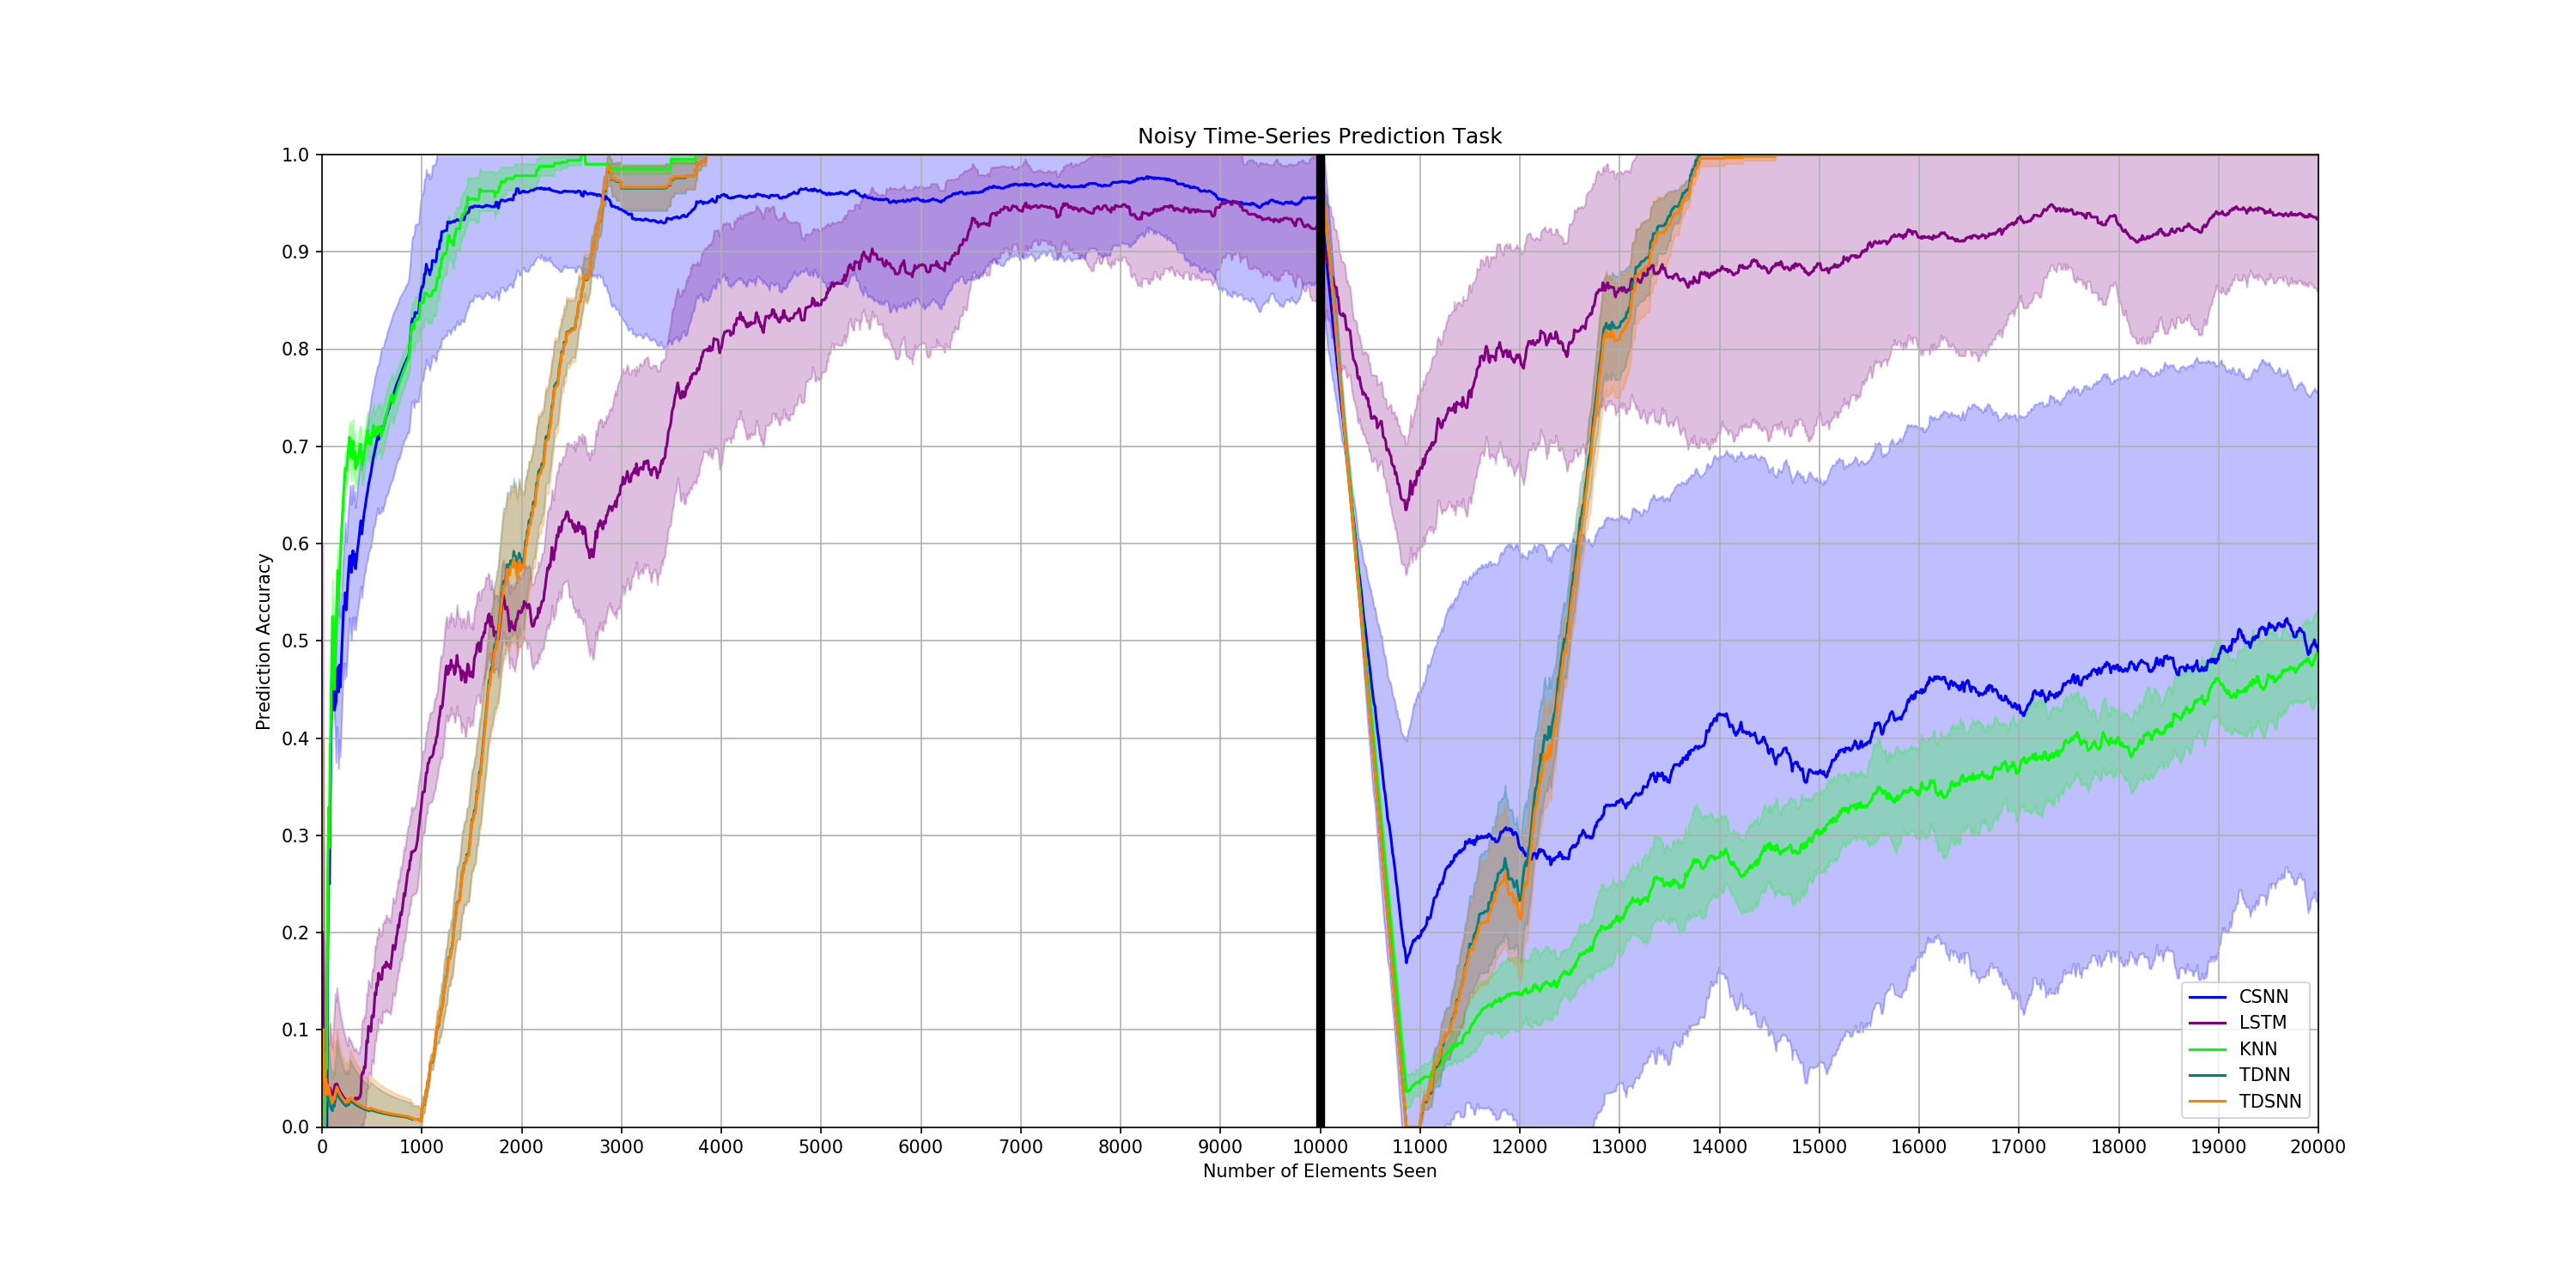
\includegraphics[width=0.9\linewidth]{../results/artificial.png}
    \caption{Each of the models were tested on their ability to predict the last element of the sequence.}
    \label{fig:prediction-accuracy}
\end{figure}

The CSNN prediction accuracy dramatically drops after the sequence endings are swapped. To improve performance, we can use a window for the data samples in the KNN Classifier. Furthermore, the learning rates for the Hebbian updates could be more carefully chosen.

\subsection*{Perturbation}

Another important property of each of these models is the robustness to temporal noise. We introduce an $\alpha$ parameters which represents the probability that a character is swapped for another character. 

%\subsection*{Continuous Dataset}

\section*{Conclusion}



\newpage
\printbibliography[title={References}]
\end{document}
